\documentclass[a4paper, twocolumn, 10pt]{IEEEtran}
 
\usepackage[utf8]{inputenc}
\usepackage[T1]{fontenc}
\usepackage{float}
\usepackage{hyperref}
\usepackage{graphicx}
\usepackage{booktabs}
 
 
\title{Servicios sí, topología no: qué replica un agente LLM del dataset Cloudscape y por qué el prompt engineering no cierra la brecha}
\author{Steven Martinez, Melissa Cobos}
\begin{document}
\maketitle
 
\begin{abstract}
Construir a mano un catálogo de arquitecturas en la nube a partir de videos toma
meses de trabajo especializado. Ese costo explica que Cloudscape, el mayor
inventario público de diseños sobre AWS con casi 400 casos, se haya quedado sin
actualizar. Este artículo mide hasta qué punto un sistema automático puede hacer
esa tarea. Reconstruimos 321 arquitecturas ya catalogadas con dos sistemas
independientes y comparamos cada resultado con la versión humana. Ninguno de los
dos sustituye al anotador: la configuración de dos etapas (Standard) reproduce el
inventario de servicios con un F1 de 86,78\,\% y las conexiones con 59,65\,\%, y
la de una sola llamada (Parsimonious) obtiene 85,73\,\% y 57,01\,\%. Esa distancia
de 27 puntos entre identificar servicios y reconstruir conexiones se mantiene en
los dos sistemas, y no se cierra reescribiendo las instrucciones: once variantes
de \emph{prompt} caben en 3,61 puntos, del tamaño de lo que el sistema varía por
sí solo. Tampoco es un problema de leer bien la pizarra, porque una persona
transcribiéndola aporta apenas 2,27 puntos. Al sustituir el catálogo curado a
mano por el nuestro en un estudio ya publicado, su clasificación coincide en el
94,8\,\% de los casos y sus rankings se preservan, pero las cifras que dependen de
flujos caen alrededor de un 28\,\%. La extracción automática ya sirve para
preguntas que dependen del conjunto de servicios; las que dependen de flujos
siguen necesitando revisión humana.
\end{abstract}
 
\section*{Palabras clave}
Arquitecturas de software, modelos multimodales, cloud, varianza de prompts.
 
 
 
\section{Introducción}
 
Las decisiones de diseño de los sistemas cloud que están en producción casi nunca
se publican. Un lugar donde sí aparecen es la serie de vídeos \emph{This is My
Architecture} de AWS, en la que un ingeniero dibuja en una pizarra el sistema que
su empresa tiene funcionando y lo explica en pocos minutos. Cloudscape convirtió
396 de esos vídeos en grafos formales y los usó para responder con datos
preguntas que antes se contestaban por intuición: qué servicios se usan de
verdad, con qué se conectan, cuánta variedad hay~\cite{satija2025cloudscape}. El
dataset ya sirve de base a otros trabajos~\cite{santillan2025hpc}.
 
Construirlo costó más de 18 persona-meses de trabajo de seis anotadores, del
orden de un día de trabajo por arquitectura. Ese costo tiene una consecuencia
concreta: el dataset se cerró en 2023 y no se ha vuelto a actualizar, aunque la
serie siguió publicando vídeos. Cualquier conclusión que hoy se extraiga de él
describe el estado de la práctica de hace varios años, y el trabajo derivado
hereda la misma fecha de corte.
 
La pregunta natural es si un agente multimodal puede hacer ese trabajo. La
respuesta que encontramos no es un sí ni un no, y es la contribución de este
artículo: \textbf{el agente reproduce el inventario de servicios y no reproduce
las conexiones entre ellos}. Sobre 321 arquitecturas comunes a dos sistemas
independientes, el F1 de servicios es 86,78\,\% y el de conexiones 59,65\,\%. Los
27 puntos que separan una cosa de la otra se mantienen en los dos sistemas, con
la misma entrada y el mismo modelo, así que no son propios de una implementación.
 
\paragraph{Qué medimos y por qué} Que el sistema sea \emph{bueno} no se decide
con una sola cifra de calidad. El catálogo se usa para responder dos clases de
preguntas distintas, y cada una depende de una magnitud distinta: las preguntas
de inventario (qué servicios se usan, con qué frecuencia) dependen del conjunto
de servicios, y las preguntas de flujo (cómo se mueven los datos, cuántos pasos
tiene un proceso) dependen de las conexiones. Por eso reportamos las dos por
separado y nunca su promedio, y por eso la conclusión del artículo es un criterio
sobre qué preguntas admiten extracción automática y cuáles no.
 
\paragraph{Lo que aporta este trabajo} Son cuatro resultados:
 
\begin{enumerate}\itemsep3pt
\item \textbf{Caractizar la asimetría} entre identificar servicios y
reconstruir conexiones, y mostramos que el déficit no es ruido sino subdibujado
sistemático, estable en dos diseños de sistema que difieren en casi todo lo
demás.
\item \textbf{Mostrar que reescribir el prompt elegido no cierra esa brecha}, y
lo establecemos contra un piso de ruido medido y no asumido. Once variantes
evaluadas sobre el mismo panel caben en 3,61 puntos, ninguna de las 55
comparaciones entre ellas sobrevive a la corrección por comparaciones múltiples,
y cuatro intervenciones diseñadas a partir del análisis de error tampoco mueven
la aguja, incluso cuando se verifica que sus mecanismos funcionan.
\item \textbf{Localizar el cuello de botella} con un experimento de tres brazos
que cambia una sola cosa: de dónde sale la descripción de la pizarra que recibe
la segunda etapa. Una persona transcribiendo el diagrama a mano no mejora el
resultado de forma detectable; entregar la referencia como entrada sí. El límite
no está en leer la pizarra, sino en que la pizarra no contiene la topología: el
52\,\% del déficit corresponde a información que solo existe en la narración o en
las convenciones de anotación del dataset.
\item \textbf{Medir qué le pasa a un estudio ya publicado} si sus datos se
reemplazan por los nuestros. Replicamos el análisis de Santillán y
Abad~\cite{santillan2025hpc} sustituyendo el conjunto de arquitecturas curado a mano y ejecutando su
código sin modificarlo: la clasificación coincide en 365 de 385 arquitecturas
(94,8\,\%) y sus rankings de servicios se preservan, mientras que las cifras que
dependen de flujos caen un 28\,\% aunque la conclusión cualitativa sobreviva.
Además el pipeline aporta 61 arquitecturas que Cloudscape no contiene, 33 de
ellas de 2024.
\end{enumerate}
 
Como subproducto metodológico documentamos una trampa que creemos general más
allá de este dominio. Al ampliar el panel de selección de 14 a 30 arquitecturas,
el ranking de variantes se invierte, y cuanto mejor puntuaba una variante en el
panel chico, más perdió al ampliarlo. Nuestra propia fase de selección de
\emph{prompts} operó por debajo de su umbral de detección, y lo reportamos como
tal.
 
El resto del artículo describe primero el sistema, el conjunto de datos y el protocolo de
evaluación, incluida la calibración del ruido que hace interpretables todas las
cifras posteriores; después presenta la evaluación; y cierra situando el trabajo
frente al trabajo relacionado, declarando las amenazas a la validez y resumiendo
la recomendación práctica.
 
\section{Motivación}
% Problema real justificado para un lector general de sistemas.
Cuando un equipo de ingeniería diseña una plataforma moderna, recurre a arquitecturas compuestas por decenas de servicios en la nube. Conocer qué patrones funcionan en producción es fundamental, pero las empresas rara vez publican sus diagramas internos. Una excepción son los vídeos técnicos (como la serie This is My Architecture), donde ingenieros dibujan y explican sus sistemas reales frente a una pizarra. El problema radica en que existen cientos de horas de conocimiento tecnológico atrapado en vídeos, y la forma actual de consultarlo es que un humano mire y pause cada grabación manualmente para copiar el diseño.
 
La evidencia de que este cuello de botella manual es un problema se encuentra en la creación del conjunto de datos Cloudscape (FAST '25). Para transcribir apenas 400 de estos vídeos en grafos formales, se requirieron más de 18 meses-persona de trabajo iterativo entre seis anotadores. Debido a este costo, el conjunto de datos dejó de actualizarse a finales de 2023. Como resultado, la comunidad académica e industrial carece de repositorios actualizados, perdiendo el rastro de las innovaciones recientes porque mantener la base de datos a mano no es viable.
 
Para un sistema automatizado, extraer estos grafos va más allá de simplemente reconocer logos en un fotograma. Primero, el reto físico de oclusión: el presentador bloquea el diagrama mientras habla, dejando la pizarra despejada solo por breves instantes. Segundo, hay desconexión multimodal: muchas conexiones se mencionan en voz pero nunca se dibujan, y contenedores genéricos nombrados visualmente como "AWS" esconden múltiples servicios mencionados en el audio. Finalmente, anotar no es transcribir: el sistema automático no debe hacer una copia literal de la pizarra, sino aplicar reglas de codificación para decidir cuándo apegarse estrictamente a la línea dibujada y cuándo usar el contexto hablado, evitando alucinar componentes ajenos al diseño.
 
\section{Metodología}
% Decisiones de diseño y detalles suficientes para replicar el trabajo.
 
El sistema toma la URL de un vídeo y devuelve un archivo .graphml con el esquema de Cloudscape. Descarga con yt-dlp, transcribe el audio con Whisper sobre GPU, extrae un fotograma cada 10 segundos, elige el mejor fotograma de pizarra y lo envía junto con la transcripción completa a un agente de dos etapas. Todo lo anterior al agente es local y no consume cuota de API, lo que permite preprocesar el catálogo entero antes de gastar llamadas. 
 
\subsection{Qué es un buen fotograma y cómo se elige}
 
De las decenas de fotogramas que da un vídeo, no todos son candidatos. El que buscamos es el que reúne tres cosas a la vez: que muestre la mayor cantidad de servicios dibujados, que muestre la mayor cantidad de líneas entre ellos, y que tenga la menor oclusión, porque el presentador está delante de la pizarra durante casi todo el vídeo. Las tres se miden por separado y se combinan en un puntaje; gana el fotograma con el puntaje más alto. 
 
\paragraph{Servicios} Los iconos de AWS son cuadros de color sobre un fondo neutro. El selector busca regiones de color vivo, aproximadamente cuadradas y de un tamaño mínimo, y confirma cada candidata comparando el brillo dentro del cuadro con el de un marco de veinte píxeles a su alrededor: si la diferencia es suficiente, hay un objeto dibujado y no una mancha del fondo. Cada icono confirmado suma puntos, y un fotograma sin ningún icono confirmado se descarta. 
 
\paragraph{Líneas} Sobre la misma zona, y tapando primero los iconos ya detectados para no contarlos dos veces, se mide cuánto trazo hay con un detector de bordes. Más trazo significa más conexiones dibujadas. El aporte de esta parte tiene un tope, para que un fotograma con ruido visual no gane solo por tener muchos bordes. 
 
\paragraph{Oclusión} Se mide qué proporción de esa zona corresponde a tonos de piel y se resta del puntaje. Es el término con más peso de los tres: un fotograma con el diagrama completo pero con el presentador delante no sirve. 
\paragraph{Sobre qué parte de la imagen se mide} El selector no recorta ni modifica el fotograma que se envía al modelo, que va completo. Lo que hace es delimitar la zona donde está la pizarra (la franja central de la imagen, dejando fuera los bordes y el pie de pantalla) y hacer ahí las tres mediciones, de modo que el fondo del plató no contamine ninguna de ellas. 
 
\paragraph{En qué parte del vídeo se busca} Se descarta el primer 20\,\% y se puntúan todos los fotogramas restantes. El diagrama se va completando a medida que el arquitecto habla, así que lo habitual en esta serie es que los mejores momentos estén hacia el final; pero no se impone como regla, porque hay vídeos donde el fotograma más completo y despejado está antes, y en esos casos es ese el que gana. Antes de puntuar se descartan además las pantallas de créditos y cierre, que el filtro reconoce por su patrón de bordes.
 
\subsection{Dos configuraciones}
La configuración Standard divide el proceso en dos pasos para simplificar el trabajo: en la etapa 1, el sistema se limita a observar y hacer un inventario exacto y literal de lo que ve (cajas, líneas y flechas) y escucha (transcripción), sin interpretar nada ni corregir errores. En la parte 2, se toma este inventario básico y se le aplica la lógica del negocio: se corrigen y normalizan los nombres de los servicios según el catálogo oficial (Cloudscape), se agrupan o separan elementos según su función, se organizan las conexiones en flujos ordenados con números de secuencia y se detallan los servicios específicos que van dentro de cada contenedor genérico.
 
La división de esta etapa se diseñó porque cuando un solo modelo intenta observar y razonar a la vez, tiende a inventar elementos que espera encontrar en lugar de ajustarse a lo que realmente está dibujado; además, separarlas ayuda a identificar si un fallo se debe a un error visual o de lógica, aunque cuesta el doble de llamadas a la API. 
 
Una alternativa más directa y económica, la configuración parsimoniosa realiza todo en una sola llamada, pero bajo reglas más estrictas: exige pruebas visuales para cada componente y se prohíbe asumir o inventar rutas de regreso que no estén dibujadas.
 
Como nota, ambas configuraciones usan el parametro de temperatura en 0 para asegurar que el modelo no sea creativo y entregue respuestas lo más precisas, consistentes y repetibles posible.
 
\subsection{Conjunto de evaluación}
Cloudscape tiene 396 arquitecturas. Se descartan las 56 que sus propios autores marcan como no utilizables, con el mismo criterio del artículo original. De las restantes, Standard logró procesar 370 y Parsimonious 385, y hay 370 que los dos procesaron. De esas, 321 dan un grafo utilizable en los dos sistemas, y son las que usamos para los resultados. Que sean las mismas 321 en los dos sistemas importa. Las arquitecturas varían mucho en dificultad: algunas tienen cuatro servicios y un diagrama limpio, otras tienen veinte y media pizarra tapada. Si cada sistema se midiera sobre un conjunto distinto, la diferencia entre sus promedios podría venir de que a uno le tocaron casos más fáciles. Al comparar arquitectura por arquitectura, esa diferencia de dificultad se cancela.
 
Los experimentos que necesitan repetir mediciones, las comparaciones entre variantes de \emph{prompt} y el experimento de oráculo, no se hacen sobre las 321 sino sobre un subconjunto fijo de \textbf{30 arquitecturas}, al que llamamos el panel. Procesar el panel una vez son 30 llamadas al modelo, y el nivel gratuito de la API admite 20 llamadas por proyecto y día. Comparar once variantes sobre las 321 arquitecturas sería inviable: el tamaño del panel lo fija esa cuota, no una decisión de diseño.
 
\subsection{Protocolo de evaluación}
La precisión se evalúa con tres indicadores: el F1 de servicios, que mide si el modelo identifica los tipos de herramientas presentes (como EC2 o RDS) sin importar sus repeticiones; el F1 de conexiones, que valida las relaciones de origen y destino entre servicios, contando cada línea de forma individual si existen flujos paralelos; y la exactitud de tipo, que calcula qué porcentaje de las conexiones correctas lleva además el tipo de arista correcto (Cloudscape distingue aristas \texttt{data}, que transportan datos, de aristas \texttt{meta}, que indican disparadores y confirmaciones). Esto ayuda a separar el qué se conecta con qué de identificar cómo se comunican.
 
Sobre esos indicadores se aplican dos protocolos de puntuación. El \textbf{protocolo estricto} mide el F1 de servicios sobre el conjunto de tipos de servicio presentes, con coincidencia exacta de cadena y sin contar repeticiones, y el F1 de aristas sobre el multiconjunto de pares dirigidos (origen, destino), contando cada línea individualmente cuando existen flujos paralelos.
 
El \textbf{protocolo permisivo} perdona tres cosas a la vez: (i) colapso de subtipos de actor (todo \texttt{User*} cuenta como \texttt{User}); (ii) aristas como conjunto, sin contar instancias duplicadas del mismo par; (iii) aristas no dirigidas, con lo que los errores de dirección dejan de penalizar. Los dos protocolos puntúan los mismos grafos generados; no hay una segunda llamada a la API.
 
 
Supóngase una arquitectura cuya referencia tiene cuatro conexiones y de la que el sistema extrae tres: 
 
\begin{itemize}\itemsep2pt
\item \texttt{UserConsumerWebMobile}$\rightarrow$\texttt{CloudFront}: el sistema
puso ahí otro subtipo de usuario, \texttt{UserCompanyDeveloper}.
\item \texttt{Lambda}$\rightarrow$\texttt{S3}: la extrajo bien.
\item \texttt{S3}$\rightarrow$\texttt{Lambda} (la respuesta de vuelta): no la
extrajo.
\item \texttt{ApiGateway}$\rightarrow$\texttt{Lambda}: la extrajo invertida,
\texttt{Lambda}$\rightarrow$\texttt{ApiGateway}.
\end{itemize}
 
 
El sistema se equivocó de tres maneras distintas: eligió un subtipo de usuario que no era, se saltó la flecha de vuelta entre \texttt{S3} y \texttt{Lambda}, y dibujó invertida la conexión con \texttt{ApiGateway}. Con el protocolo estricto acierta 1 de 4. La regla (i) perdona el subtipo de usuario y lo lleva a 2 de 4. La regla (ii) hace que las dos flechas entre \texttt{Lambda} y \texttt{S3} cuenten como una sola, así que la referencia pasa a tener 3 conexiones en vez de 4. La regla (iii) da por buena la flecha invertida de \texttt{ApiGateway}. El resultado final es 3 de 3.
 
Esa última consecuencia obliga a un uso restringido del protocolo: bajo la regla (iii) un sistema que invirtiera todas las flechas obtendría un F1 de aristas perfecto. El permisivo sirve para localizar dónde está el error, nunca para acreditar qué tan bien se reconstruyen las conexiones; este artículo contiene más del protocolo estricto.
 
La Figura~\ref{fig:permisivo} muestra el efecto de las tres reglas sobre el panel de 30. En servicios toda la ganancia viene de la primera regla, que es una corrección de nomenclatura y hace que el sistema acierte más. En aristas la mayor parte viene de la tercera, que no añade aciertos sino que achica la referencia contra la que se compara.
 
 
\begin{figure}[H]
\centering
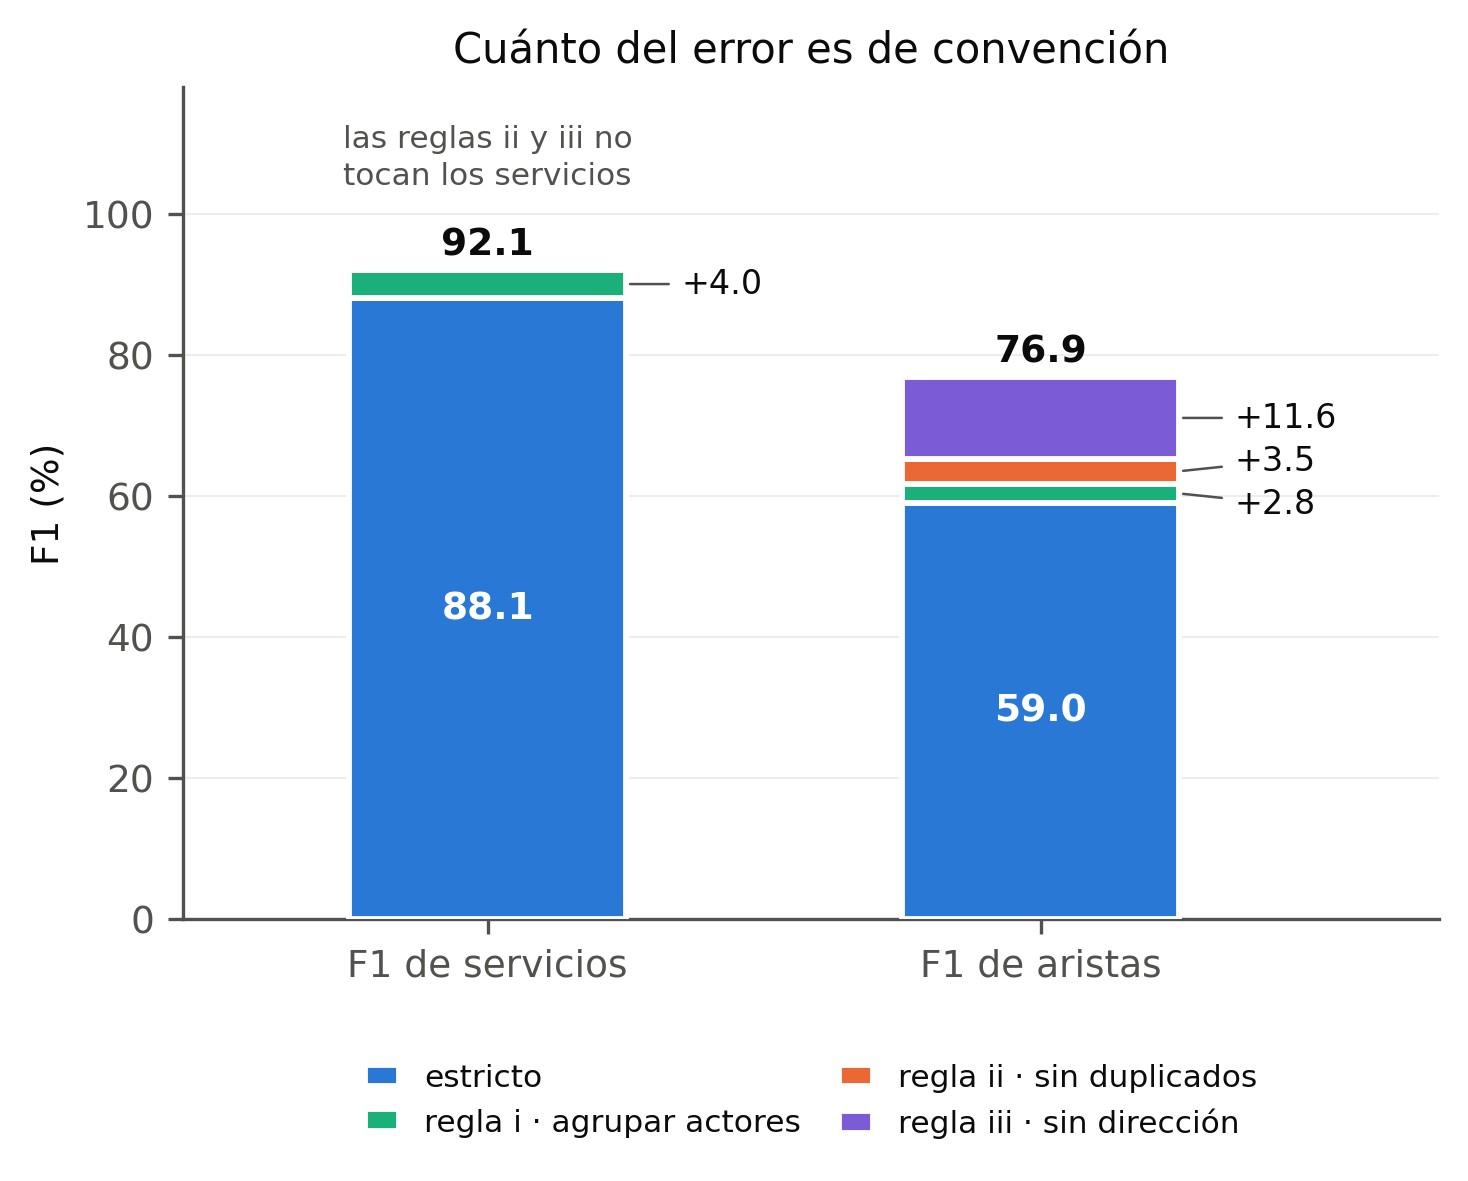
\includegraphics[width=\columnwidth]{imgs/fig5_permisivo_3reglas.png}
\caption{Protocolo estricto frente al permisivo. La ganancia proviene en su mayor parte de que la referencia se achica, no de más aciertos.}
\label{fig:permisivo}
\end{figure}
 
% aqui hay q poner algo referente a la figura 1 del paper
 
\subsection{Cuánto varía el sistema por sí solo}
\label{sec:piso}
 
Un modelo de lenguaje no devuelve siempre lo mismo ante la misma entrada, ni siquiera con la temperatura en cero. Si se corre el sistema dos veces sin cambiar nada, los dos resultados difieren un poco. A esa variación propia la llamamos el piso de ruido, y hay que medirla antes de cualquier comparación: sin ella no se puede saber si una diferencia entre dos configuraciones significa algo o si es del tamaño de lo que el sistema se mueve solo. A temperatura $0{,}0$, \textbf{0 de 170} salidas repetidas fueron idénticas carácter por carácter, así que la variación existe y hay que acotarla.
 
% Esa dispersión, que anotamos $\sigma_d$, es la de la Tabla~\ref{tab:mde}, y de ella sale el efecto mínimo detectable: la diferencia más pequeña que el diseño puede distinguir del ruido, que se aproxima por 
 
% \begin{equation}
% \mathrm{MDE} \;\approx\; 2{,}8\,\frac{\sigma_d}{\sqrt{n}}
% \qquad (\alpha = 0{,}05 \text{ bilateral},\ \text{potencia } 0{,}80).
% \end{equation}
 
% \begin{table}[t]
% \centering\small\setlength{\tabcolsep}{4pt}
% \caption{Piso de ruido medido sobre réplicas nulas del panel de 30.}
% \label{tab:mde}
% \begin{tabular}{lrrr}
% \toprule
% Métrica & $\sigma_d$ & $\mathrm{MDE}_{n=14}$ & $\mathrm{MDE}_{n=30}$\\
% \midrule
% F1 de aristas     & 6,43 & 4,81 & \textbf{3,29}\\
% F1 de servicios   & 3,45 & 2,58 & \textbf{1,76}\\
% Aristas generadas & 1,42 & 1,06 & 0,73\\
% Nodos generados   & 0,66 & 0,50 & 0,34\\
% \bottomrule
% \end{tabular}
% \end{table}
 
\subsection{Repositorio}
El código del pipeline, los grafos generados y los prompts de evaluación están en el repositorio del proyecto en el siguiente enlace:
\url{https://github.com/stevenijm777/aws-architecture-extraction}
 
\section{Results / Evaluation}
% Métricas adecuadas, rango de parámetros y conclusiones de la data.

Respondiendo a la pregunta de la introducción sobre si la extracción automática puede ampliar un repositorio de arquitecturas cloud, este estudio empírico encuentra una respuesta partida. A nivel de servicios el sistema alcanza 86,78 de F1 bajo el protocolo estricto. A nivel de conexiones se queda en 59,65, y el déficit es sistemático: el número de nodos es correcto y el de aristas queda por debajo del de la referencia. El sistema reproduce qué componentes forman una arquitectura, no cómo se conectan.

\subsection{Servicios frente a conexiones}
\label{sec:rq1}

\begin{table}[H]
\centering\small
\caption{Desempeño sobre las 321 arquitecturas comunes a los dos sistemas
(protocolo estricto).}
\label{tab:rq1}
\begin{tabular}{lrrr}
\toprule
 & Standard & Parsimonious & Ref.\\
\midrule
F1 de servicios & 86,78 & 85,73 & ---\\
F1 de aristas   & 59,65 & 57,01 & ---\\
Brecha          & \textbf{27,13} & \textbf{28,72} & ---\\
\midrule
Nodos por arq.   & 9,15 & 9,33 & 9,11\\
Aristas por arq. & 9,04 & 8,83 & 12,42\\
\bottomrule
\end{tabular}
\end{table}

La Tabla~\ref{tab:rq1} contiene el resultado central. La distancia entre
identificar servicios y reconstruir conexiones es de 27 puntos y se
mantiene en dos diseños de sistema independientes —dos etapas con formato
de salida forzado frente a una sola llamada con lector escrito a mano—
que difieren en casi todo lo demás, de modo que no es un artefacto de una
configuración.

Los conteos muestran que el déficit no es una pérdida difusa de
precisión. Los nodos calzan: 9,15 generados contra 9,11 del \emph{ground
truth}, una diferencia muy por debajo del umbral de detección
($0{,}12\times$ el MDE). Las aristas se subdibujan: 9,04 generadas contra
12,42, un déficit de $-3{,}38$ por arquitectura que es 4,7 veces ese
umbral. El agente reconstruye el inventario correcto de componentes y
dibuja menos conexiones de las que hay. La Figura~\ref{fig:asimetria}
muestra esa asimetría arquitectura por arquitectura y la
Figura~\ref{fig:subdibujado} la separa en sus dos conteos.

\begin{figure}[H]
\centering
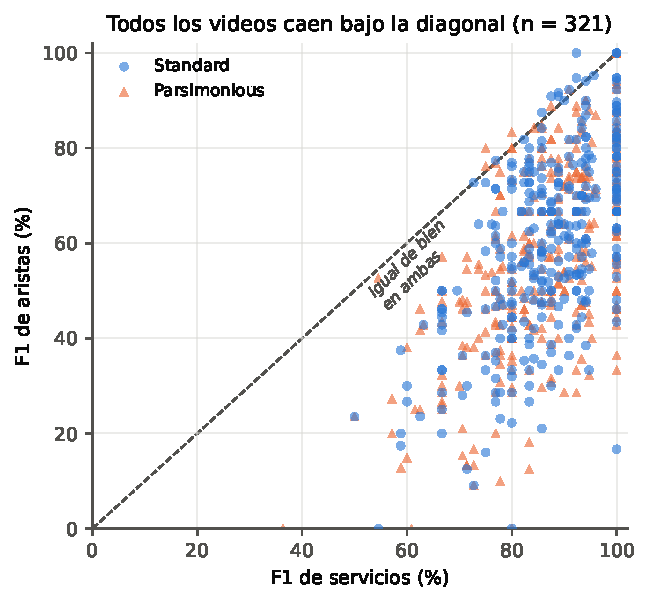
\includegraphics[width=\columnwidth]{imgs/fig1_asimetria_servicios_vs_aristas.pdf}
\caption{F1 de servicios frente a F1 de aristas por arquitectura ($n=321$). La
nube completa cae por debajo de la diagonal.}
\label{fig:asimetria}
\end{figure}

\begin{figure}[H]
\centering
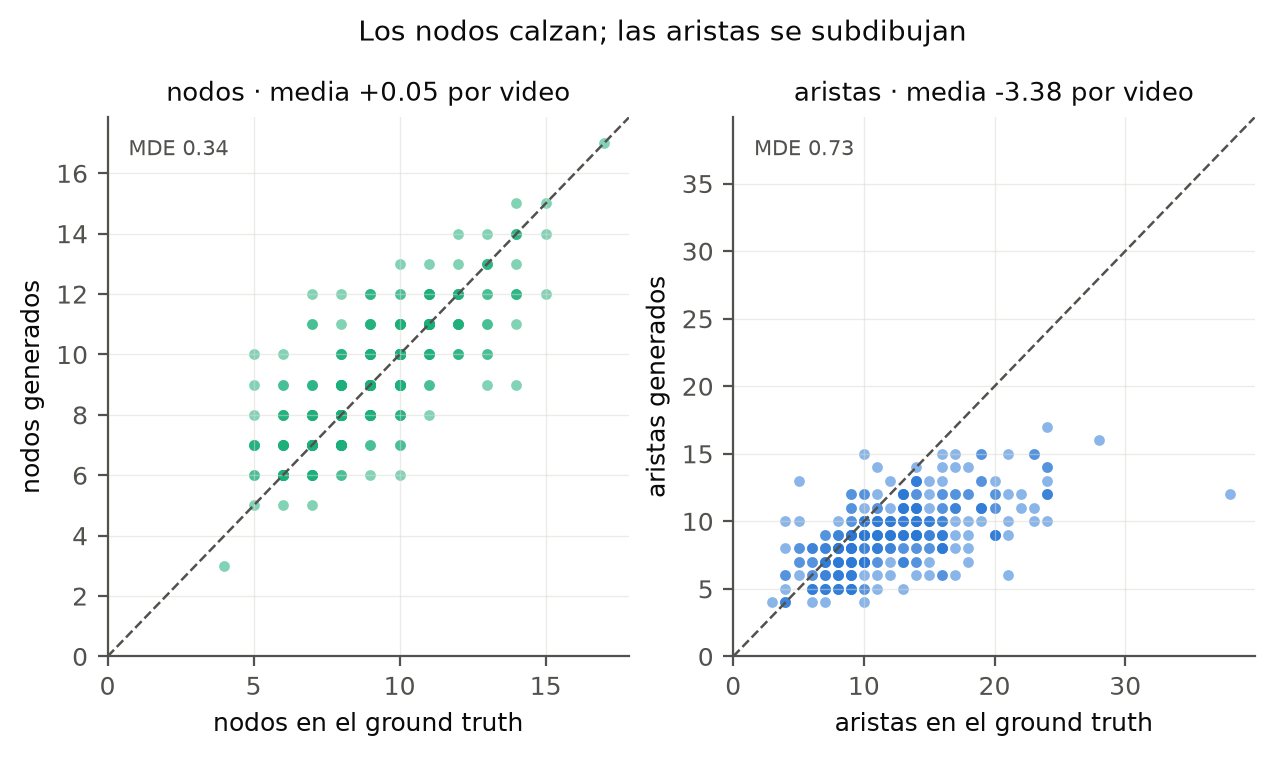
\includegraphics[width=\columnwidth]{imgs/fig2_subdibujado.png}
\caption{Nodos generados frente a nodos del \emph{ground truth} (izquierda) y
aristas generadas frente a aristas del \emph{ground truth} (derecha). Los nodos
calzan; las aristas quedan por debajo en $-3{,}38$ por arquitectura.}
\label{fig:subdibujado}
\end{figure}

\paragraph{Standard frente a Parsimonious.} La comparación se hace sobre
cada arquitectura por separado, y el resultado es partido. En servicios
Standard aventaja a Parsimonious por 1,05 puntos, pero la evidencia no es
concluyente: las dos pruebas no paramétricas caen a lados opuestos del
umbral (signos $p=0{,}049$; Wilcoxon $p=0{,}066$) y 159 de las 321
arquitecturas obtienen el mismo puntaje en las dos configuraciones, así
que la mitad de la muestra no aporta información. En aristas la
diferencia es de 2,64 puntos, las dos pruebas coinciden
($p=0{,}00026$ y $p=0{,}00006$) y el intervalo de confianza no toca el
cero. La configuración de una sola llamada rinde igual en servicios y
peor al reconstruir las conexiones.

\subsection{La variación del \emph{prompt} en Standard}
\label{sec:rq2}

\begin{table}[H]
\centering\small
\caption{Once variantes de \emph{prompt} de la etapa 2 sobre el panel de 30.}
\label{tab:variantes}
\begin{tabular}{lrr}
\toprule
Variante & F1 servicios & F1 aristas\\
\midrule
V7 retorno sobre V6 (c10)          & 88,07 & \textbf{60,10}\\
V6 optimizado (c8)                 & 86,75 & 59,14\\
V6 corregido (c9) --- producción   & 88,06 & 58,99\\
V7 flujos de retorno (c7)          & 86,91 & 58,65\\
V5 ruteo estricto (c8)             & 86,78 & 58,45\\
V8 actores y retornos              & 86,21 & 58,40\\
V6 corregido (c10)                 & 88,47 & 58,10\\
V5 ruteo estricto (c7)             & 86,65 & 58,08\\
V6 corregido (c7)                  & 85,92 & 57,52\\
V4 anti-alucinación (c8)           & 85,62 & 57,10\\
V4 \emph{few-shot} dinámico        & 88,03 & 56,49\\
\midrule
\textbf{Rango}                     & \textbf{2,84} & \textbf{3,61}\\
MDE ($n=30$)                       & 1,76 & 3,29\\
\bottomrule
\end{tabular}
\end{table}

La Tabla~\ref{tab:variantes} recoge once variantes evaluadas en las
mismas condiciones: mismo panel, mismo modelo, misma temperatura y las
mismas imágenes de pizarra. Entre la mejor y la peor hay 3,61 puntos de
F1 de aristas, apenas por encima de los 3,29 que el sistema se mueve
solo.

Ese margen acota lo que el diseño \emph{podría} detectar; lo que
efectivamente detecta lo dicen las pruebas pareadas. Comparar el extremo
mejor contra el peor da 10 victorias, 7 derrotas y 13 empates
($p=0{,}629$), y sin corregir apenas 3 de las 55 comparaciones bajan de
$p=0{,}05$.

Siguiendo a Arcuri y Briand~\cite{Arcuri2011StatisticalSE}, el argumento
no descansa en el $p$ sino en el tamaño de efecto con su intervalo de
confianza, que es lo que distingue \emph{no hay efecto} de \emph{no hay
potencia}. Reportamos $\hat{A}_{12}$ de Vargha y Delaney ---la medida que
esos autores recomiendan para escala de intervalo--- con intervalo por
\emph{bootstrap} sobre arquitecturas.

\begin{table}[H]
\centering\small
\caption{Tamaños de efecto sobre las 55 comparaciones entre variantes.}
\label{tab:a12}
\begin{tabular}{lr}
\toprule
Sobre las 55 comparaciones & Valor\\
\midrule
Rango de $\hat{A}_{12}$            & $0{,}452 - 0{,}553$\\
Magnitud del efecto                & \textbf{insignificante en las 55}\\
IC$_{95\%}$ que contiene $0{,}5$   & \textbf{55/55}\\
Ancho medio del IC                 & $0{,}110$\\
\bottomrule
\end{tabular}
\end{table}

Cincuenta y cinco intervalos angostos centrados en $0{,}5$ no son un resultado ambiguo: acotan cuánto podría estar escondido y lo dejan cerca de cero. El contraste vive en la misma prueba y sobre el mismo panel: el brazo de oráculo de la Sección~\ref{sec:rq3} da
$\hat{A}_{12}=0{,}861$ con IC$_{95\%}$ $[0{,}794;\,0{,}927]$, un efecto grande. El diseño detecta diferencias cuando las hay. Por eso la afirmación que sostenemos es que \emph{ninguna diferencia entre variantes es detectable}, no que las variantes sean equivalentes.

Como control de robustez añadimos la corrección por comparaciones
múltiples: el $p$ mínimo es $0{,}0074$ frente a un $\alpha$ de Bonferroni de $0{,}00091$, y ninguna comparación sobrevive ni bajo Bonferroni ni bajo Holm. Lo reportamos para mostrar que la conclusión no depende de esa elección, no como su fundamento: los propios Arcuri y Briand desaconsejan Bonferroni por conservador y por inflar el error de Tipo~II.

\paragraph{Cuatro intervenciones dirigidas, cuatro resultados nulos.}
La invarianza no se limita a reescrituras superficiales del
\emph{prompt}. Diseñamos cuatro intervenciones a partir de los errores
más frecuentes observados en las salidas del sistema, todas medidas
sobre el mismo panel contra la misma línea base (88,06 servicios /
58,99 aristas).

\begin{table}[H]
\centering\small
\caption{Intervenciones dirigidas sobre el panel de 30.}
\label{tab:intervenciones}
\begin{tabular}{lrrr}
\toprule
Intervención & $\Delta$ aristas & $\times$MDE & signos\\
\midrule
Evidencia visual (Hough)   & $-1{,}60$ & $0{,}49$ & $p=0{,}55$\\
V8 · actores y retornos    & $-0{,}59$ & $0{,}18$ & $p=0{,}61$\\
Auditoría de retornos      & $+1{,}20$ & $0{,}36$ & $p=1{,}00$\\
\emph{Few-shot} RAG        & $-2{,}50$ & $0{,}76$ & $p\approx0{,}33$\\
\bottomrule
\end{tabular}
\end{table}

Ninguna de las cuatro, recogidas en la Tabla~\ref{tab:intervenciones},
alcanza la mitad del umbral. Lo relevante es que en dos de ellas
se verificó que el mecanismo funcionó: la auditoría de retornos generó
propuestas válidas en el 100\,\% de los casos, y V8 sí recuperó nodos
actor y sí subió la bidireccionalidad. El mecanismo opera y el F1 de
aristas no se mueve. Eso es lo que descarta que la brecha sea un problema
de instrucción.

\subsection{Qué etapa limita el resultado}
\label{sec:rq3}

Este experimento se corre sobre la configuración Standard. Consiste en tres ejecuciones del sistema, que llamamos brazos, idénticas en todo (mismo \emph{prompt}; mismo modelo; mismo panel de 30) salvo en una sola cosa: de dónde sale la descripción de la pizarra que la etapa 2 recibe como entrada.

\begin{itemize}\itemsep2pt
\item \textbf{Producción}: la descripción la genera la etapa 1, como en el uso
normal del sistema.
\item \textbf{Brazo A}: la escribió una persona mirando solo la pizarra, sin
escuchar el audio y sin ver el \emph{ground truth}.
\item \textbf{Brazo B}: es el \emph{ground truth} de Cloudscape, es decir, la
respuesta correcta entregada directamente como entrada.
\end{itemize}

La lógica es de descarte: si el sistema falla porque lee mal el diagrama, darle una lectura humana debería mejorarlo; si falla por otra razón, no. La Tabla~\ref{tab:oraculos} recoge los tres brazos.

\begin{table}[H]
\centering\footnotesize\setlength{\tabcolsep}{4pt}
\caption{Experimento de oráculo: tres brazos, panel de 30. La última columna es
la diferencia con producción, en puntos y en múltiplos del MDE: el brazo A cabe
dentro del ruido y el brazo B no.}
\label{tab:oraculos}
\begin{tabular}{lrrl}
\toprule
Brazo & F1 svc & F1 aristas & Dif.\\
\midrule
Producción (4 réplicas)  & 87,10 & 58,13 & \textemdash\\
A · transcripción humana & 87,82 & 60,40 & $+2{,}27$ (0,69$\times$)\\
B · \emph{ground truth}  & 99,57 & 82,17 & $+24{,}04$ (7,31$\times$)\\
\bottomrule
\end{tabular}
\end{table}

Si el límite del sistema fuera que la primera etapa lee mal el diagrama, el brazo A tendría que acercarse al brazo B. No se despega de producción: 17 victorias, 7 derrotas, 6 empates, $p=0{,}064$, dentro del MDE. El brazo B sí lo hace: 27 victorias, 1 derrota, $p<0{,}001$.

\paragraph{El techo de la pizarra, medido directamente.}
Lo anterior es un argumento por resta, y admite una verificación independiente que no pasa por la etapa 2: puntuar las 30 transcripciones humanas directamente contra la referencia. Eso mide qué fracción del \emph{ground truth} es siquiera recuperable mirando la pizarra, que es la cota superior de cualquier sistema que solo mire la imagen.

\begin{table}[H]
\centering\small\setlength{\tabcolsep}{4pt}
\caption{Quién lee la pizarra, panel de 30.}
\label{tab:techo}
\begin{tabular}{lrrr}
\toprule
 & F1 svc & F1 aristas & Aristas/arq.\\
\midrule
\textbf{Una persona, solo la pizarra} & \textbf{87,36} & \textbf{57,60} & 8,63\\
Pipeline completo                     & 87,10 & 58,13 & 9,03\\
\emph{Ground truth}                   & 100   & 100   & 12,03\\
\bottomrule
\end{tabular}
\end{table}

No queda margen perceptual. Una persona haciendo la tarea de percepción sin oclusión que la confunda y sin límite de tiempo recupera los servicios igual que el pipeline y las aristas igual de mal, medio punto de diferencia. Y también subdibuja: anota 8,63 aristas donde la referencia tiene 12,03, un déficit de $-3{,}40$ por arquitectura frente al $-3{,}38$ del sistema automático. El subdibujado no es un artefacto del modelo ni una carencia de instrucción: esas aristas no están dibujadas.

\paragraph{Descomposición de la brecha.}
Con esa medición, repartir los 41,87 puntos que separan producción del 100\,\% deja de ser una inferencia.

\begin{table}[H]
\centering\small\setlength{\tabcolsep}{4pt}
\caption{Descomposición de la brecha de 41,87 puntos que separa producción del techo.}
\label{tab:tramos}
\begin{tabular}{lrr}
\toprule
Tramo & Puntos & \%\\
\midrule
Etapa 1 autom. $\rightarrow$ transcr. humana & 2,27 & 5,4\\
Transcr. humana $\rightarrow$ \emph{ground truth} & 21,77 & \textbf{52,0}\\
\emph{Ground truth} $\rightarrow$ 100 & 17,83 & 42,6\\
\bottomrule
\end{tabular}
\end{table}

Es decir: la calidad de lectura de la pizarra explica el 5,4\,\% del problema. El 52\,\% corresponde a información que no está en la imagen, porque el \emph{ground truth} de Cloudscape se anotó viendo el vídeo completo, con narración, y buena parte de las aristas vive en ese canal verbal o en el criterio de anotación, no en el dibujo. El 42,6\,\% restante es pérdida propia de la segunda etapa incluso teniendo la respuesta delante, y marca el techo de esta arquitectura de agente.

\subsection{¿Sirven estos grafos en un estudio publicado?}
\label{sec:downstream}

Todo lo anterior mide el pipeline contra una referencia. Esta sección
mide si sus errores cambian las conclusiones de un trabajo real, con dos
experimentos distintos sobre corpus distintos.

\paragraph{Propagación del error.} Ejecutamos el código de Santillán y
Abad~\cite{santillan2025hpc}, que clasifica cada arquitectura como
HPC, Edge, ambas o ninguna a partir de los servicios presentes,
sustituyendo su corpus anotado a mano por los grafos que extrae nuestro
sistema sobre las mismas 385 arquitecturas que ellos ya tenían
clasificadas. Lo único que cambia es quién leyó la pizarra.

\begin{table}[H]
\centering\small
\caption{Propagación del error a la clasificación HPC/Edge (385 arquitecturas pareadas).}
\label{tab:downstream}
\begin{tabular}{lr}
\toprule
Resultado & Valor\\
\midrule
Coincidencia de clasificación     & 365/385 = 94,8\,\%\\
Ranking top-10 preservado (HPC)   & 7/10\\
Ranking top-10 preservado (Edge)  & 8/10\\
Ranking top-10 preservado (None)  & 9/10\\
\bottomrule
\end{tabular}
\end{table}

Lo que se ve en el clasificador que usa Santillán y Abad es que basta que falte un solo servicio para que una arquitectura cambie de categoría. Es el peor caso posible para nuestros errores, y aun así la clasificación coincide en 94,8\,\% de los casos. Los desacuerdos tienen una causa identificable: la mayoría se explica por un único nodo de actor perdido (un dispositivo, no un servicio de AWS), lo que es consistente con que lo que se pierde son convenciones de anotación y no servicios cloud.

Sobre la parte de ese estudio que depende de la topología, el conteo de \emph{workflows} por arquitectura, el resultado es distinto: la conclusión cualitativa de los autores (los grupos no se separan por número de \emph{workflows}) se mantiene con nuestra extracción, pero las medias caen alrededor de un 28\,\%, porque el sistema subcuenta \emph{workflows} igual que subdibuja aristas. Quien reemplace la anotación manual por este pipeline llegaría a la misma conclusión, con cifras sistemáticamente bajas.

\paragraph{Extensión del catálogo.} Por separado, el pipeline procesa 61 arquitecturas que Cloudscape no cubre, 33 de ellas de vídeos de 2024, y las clasifica con la misma regla de Santillán y Abad. Sobre esas 61 no hay anotación humana con la cual comparar, así que lo que reportamos no es acierto sino el resultado de la clasificación en sí: la proporción de arquitecturas Edge entre las 457 resultantes (las 396 originales más las 61 nuevas) pasa de 25,5\,\% a 27,4\,\%, y entre los vídeos de 2024 específicamente es del 27\,\%. Es una actualización del catálogo, no una tendencia: los propios autores advierten que la variación anual de la serie puede deberse al azar o a la curaduría del canal, y no hacen afirmaciones de representatividad sobre la nube en general. La frontera queda con una forma más precisa: lo que depende del conjunto de servicios sobrevive casi intacto; lo que depende de la topología conserva la conclusión y pierde la escala.

 
\section{Trabajo relacionado}
% Agrupación temática, novedad respecto a trabajos previos y tono constructivo.
La reconstrucción de arquitecturas de software permite recuperar los mapas de diseño de un sistema a partir de su código fuente \cite{Ducasse2009SAR}. Sin embargo, investigaciones previas demuestran que las herramientas automáticas de recuperación suelen tener un porcentaje de acierto muy bajo al agrupar componentes y definir la estructura general del sistema \cite{Garcia2013ComparativeSAR}. Esta falta de precisión justifica la decisión de evaluar los servicios de AWS y sus flechas de conexión de forma independiente en este trabajo. La principal diferencia de esta propuesta frente a los métodos tradicionales es que no analiza el código escrito, sino que extrae el diseño de forma directa desde videos técnicos en los que un expositor dibuja su arquitectura en una pizarra y la explica en voz alta.
 
 
Para poder estudiar la nube es necesario contar con datos reales sobre diseños de la industria. El dataset Cloudscape \cite{satija2025cloudscape} es un esfuerzo pionero que transforma videos explicativos de AWS en diagramas estructurados de puntos y flechas. Por otro lado, estudios sobre sistemas en producción, como los realizados sobre microservicios de Alibaba \cite{Luo2021AlibabaMicroservices}, destacan que comprender estas topologías y rutas de comunicación es clave para optimizar el rendimiento y evitar problemas de comunicación en arquitecturas complejas. Este trabajo se diferencia al automatizar la obtención de estos mapas directamente a partir de un video explicativo, introduciendo además una métrica que califica el resultado contando cada flecha de manera individual para castigar las conexiones falsas inventadas por el modelo.
 
Las dificultades que enfrentan los modelos de lenguaje al procesar datos estructurados están documentadas. Se ha mostrado que la capacidad de razonamiento de estas herramientas disminuye mucho al analizar grafos o mapas con conexiones densas y cruzadas \cite{Fatemi2024TalkLikeAGraph, Wang2023NLGraph}. Estas limitaciones respaldan los hallazgos de este estudio: la diferencia entre el diagrama real y el mapa generado por la computadora no se soluciona simplemente cambiando las palabras de las instrucciones. Esta literatura llevaría a esperar que el límite de un sistema como este estuviera en el modelo, y que mejorarlo pasara por ajustar la forma de pedirle la tarea. El aporte de este trabajo es poner esa expectativa a prueba en lugar de asumirla, mediante variantes de instrucción y experimentos que sustituyen
una etapa del sistema a la vez.
 
 
Para garantizar que las fallas de conexión detectadas se deben a límites del modelo y no a errores del sistema propuesto, se utilizaron técnicas de evaluación probadas. Se implementó una estrategia tipo oráculo similar a la propuesta en reparación de software \cite{Liu2019FaultLocalizationBias}, la cual asume temporalmente que una de las fases del proceso funciona perfectamente para poder aislar y medir el rendimiento real de las demás etapas. Asimismo, para evitar conclusiones apresuradas, el análisis se apoya en guías de evaluación estadística recomendadas para ingeniería de software \cite{Arcuri2011StatisticalSE} y en la evaluación con múltiples variantes de instrucciones \cite{Mizrahi2024MultiPromptEval}. Esto permite demostrar que las pequeñas variaciones en los resultados de los modelos son producto de su sensibilidad al texto utilizado y no de mejoras reales en el diseño.


 
 
\section{Conclusiones}
% Interpretación de resultados, trabajo futuro.
% Enlace al repositorio de código:
% \url{https://github.com/usuario/repo}
Este trabajo muestra que se puede extraer de forma automática diagramas de arquitectura en la nube a partir de videos explicativos que combinan imagen y audio. La principal conclusión del estudio es que, para procesar diagramas complejos de manera precisa, es necesario separar el observar la imagen del razonamiento técnico. La configuración de dos pasos (Standard) alcanza un F1 de servicios del 86,78\,\% y de conexiones del 59,65\,\%. Frente a la de un solo paso (Parsimonious), su ventaja está establecida en las conexiones, donde la diferencia de 2,64 puntos es consistente en las dos pruebas aplicadas, y no en los servicios, donde las pruebas no coinciden y la mitad de las arquitecturas empata. Dividir la tarea ayuda, entonces, justamente donde el modelo tiene que razonar sobre el dibujo, y no donde solo tiene que nombrar lo que ve.
 
Además, los datos evidencian una relación entre el costo del sistema y la precisión del diagrama final. Aunque el enfoque de dos etapas ofrece el resultado más exacto, requiere el doble de llamadas a la API. En cambio, la opción de una sola etapa (Parsimonious) reduce a la mitad el uso de la API y el tiempo de procesamiento, perdiendo 1,05 puntos en la detección de servicios y 2,64 puntos en el trazo de conexiones. Este análisis permite elegir la configuración del sistema dependiendo de si se prioriza la máxima exactitud o el ahorro de recursos.
 
Respecto a si un agente de IA puede reemplazar al experto en el análisis de arquitecturas en la nube, los resultados de la propuesta indican que no es posible una sustitución completa. Aunque el sistema automatiza con éxito tareas visuales básicas y de transcripción, la menor precisión obtenida en el trazado de las conexiones (59,65\,\%) demuestra que la capacidad del agente tiene límites. El criterio del especialista sigue siendo indispensable para resolver ambigüedades técnicas y garantizar que el diagrama generado represente fielmente el funcionamiento real del sistema. Así, el agente actúa como un asistente para acelerar el trabajo de recolección de datos, pero no reemplaza la validación final del experto.
 
Conviene señalar además dos resultados negativos que acotan el espacio de mejora. Reescribir las instrucciones no cierra la brecha: once variantes evaluadas sobre el mismo panel caben en 3,61 puntos, del tamaño de lo que el sistema varía por sí solo, y cuatro intervenciones diseñadas a partir del análisis de error tampoco la mueven aunque se verifique que sus mecanismos funcionan. Y mejorar la lectura de la pizarra tampoco alcanza: una persona transcribiendo el diagrama a mano no despega el resultado de la ejecución automática, mientras que entregar la referencia como entrada sí lo hace. El límite, entonces, no está en ver el dibujo sino en que buena parte de la topología no está dibujada.
 
Como trabajo futuro se sugieren tres líneas. La primera es mejorar la clasificación del tipo de conexión, que hoy registra el rendimiento más bajo. La segunda es medir el acuerdo entre anotadores humanos sobre un subconjunto del dataset: todas las cifras de este trabajo se comparan contra una única anotación de referencia cuya consistencia interna se desconoce, así que hoy no es posible saber cuánto del desacuerdo es error del sistema y cuánto es la variabilidad que dos expertos tendrían entre sí. La tercera es tratar la narración del vídeo como fuente primaria y no como contexto de apoyo, ya que la mayor parte de lo que falta vive en el audio y no en la pizarra.
 
 
 
 
\bibliographystyle{ieeetr}
\bibliography{referencias}% common bib file
 
\end{document}